\pagebreak
\section{Deferred Shading}

\begin{center}
\emph{{\small Tobias Graf}}
\end{center}

\bigskip

\subsubsection*{Einleitung} Um aus der entstandenen Drahtgitter - Oberfläche des Marching Cubes Algorithmus eine Näherung zu einer Wasseroberfläche zu erzielen verwenden wir Deferred Shading. In diesem Kapitel wird kurz erläutert was Deferred Shading generell ist und wie unsere Implementierung das ganze Nutzt um einen Transparenten Wassereffekt zu erreichen.

\subsection*{Deferred Shading} Ursprünglich ist Deferred Shading eine Technik der Computergrafik um die Lichtberechnung von der Geometrieberechnung zu trennen. Sie erlaubt durch das Reduzieren der Komplexität wesentlich mehr Lichtobjekte in einer Szene als bei klassischen Rendermethoden, in denen anhand der Tiefe, Normale und Farbwert eines Eckpunktes in Korrelation einer Lichtquelle die Dargestellte Farbe berechnet wurden. Beim Deferred Shading werden durch sogenannte Framebufferobjekte (FBO) Tiefenwerte, Normale und Farbe der Geometrien in eine Textur mit Bildschirmauflösung gerendert. Statt nun für jeden Geometrischen Eckpunkt den Farbwert zu berechnen wird dies nun für jeden Pixel angewandt wodurch der Aufwand von $O(m*n)$ auf $O(m+n)$ reduziert wird. Nachteilig dabei ist das zwar weniger Hardwareanforderungen benötigt werden um die gleiche Szene zu rendern, jedoch der Speicherverbrauch extrem ansteigt da die Texturen im Grafikkartenspeicher vorgehalten werden müssen.\\
Relativ schnell Entwickelten sich vielfältige Nutzungen der Technik zur Berechnung von Shadow Maps und einsetzen von Postprocessing Effekten.

\subsection*{Unser Ansatz} Angelehnt an den Ansatz des GDC Vortrags\cite{DSGDC} erfolgte zuerst die Implementation mehrerer Framebufferobjekte die als einzelne Rendertargets benutzt werden um verschiedene Aspekte der Szene einzeln in Texturen zu Rendern. Die Aufteilung erfolgt in folgende FBO und Grafiken:
\begin{itemize}
\item Hintergrund
\item Thickness
\item Partikel
	\begin{itemize}
	\item Farbwert
	\item Tiefenwert
	\item Welt - Koordinate
	\item Normale
	\item Spekulare Farbe
	\item Diffuse Farbe
	\end{itemize}
\end{itemize}  
\medskip
\noindent Das getrennte Rendern des Hintergrundes ist notwendig um den Transparenz Effekt zu erreichen da dies eine schwäche von Deferred Shading ist da man keinen nutzen aus der \texttt{GL_BLEND} Funktion ziehen kann wenn die einzelnen Geometrien in getrennten FBO gezeichnet werden. Die Thickness bestimmt im abschließenden Bild die Hauptsächliche Transparenz der Oberfläche. Der Partikel FBO schreibt die einzelnen Parameter mit denen die Lichtberechnung des Phong Modells und die Farbgebung des Objektes in die jeweiligen Texturen.
\begin{align*}
\noindent
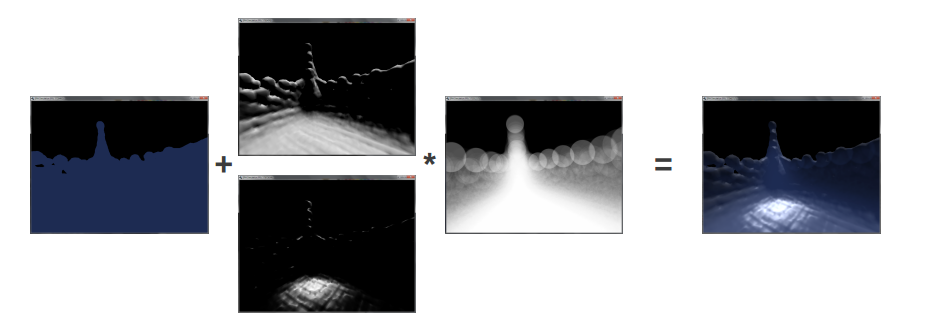
\includegraphics[scale=0.9]{images/Dereffered}
\end{align*}
\medskip  